% Requires \usepackage{subcaption} and \usepackage{graphicx}.
\begin{figure*}[t]
  \centering
  \begin{subfigure}[t]{0.245\textwidth}
    
\includegraphics[width=\linewidth]{experiments/annotation_viz/output/page_10_no_annotations.png}
    \caption{Original image}
  \end{subfigure}\hfill
  \begin{subfigure}[t]{0.245\textwidth}
    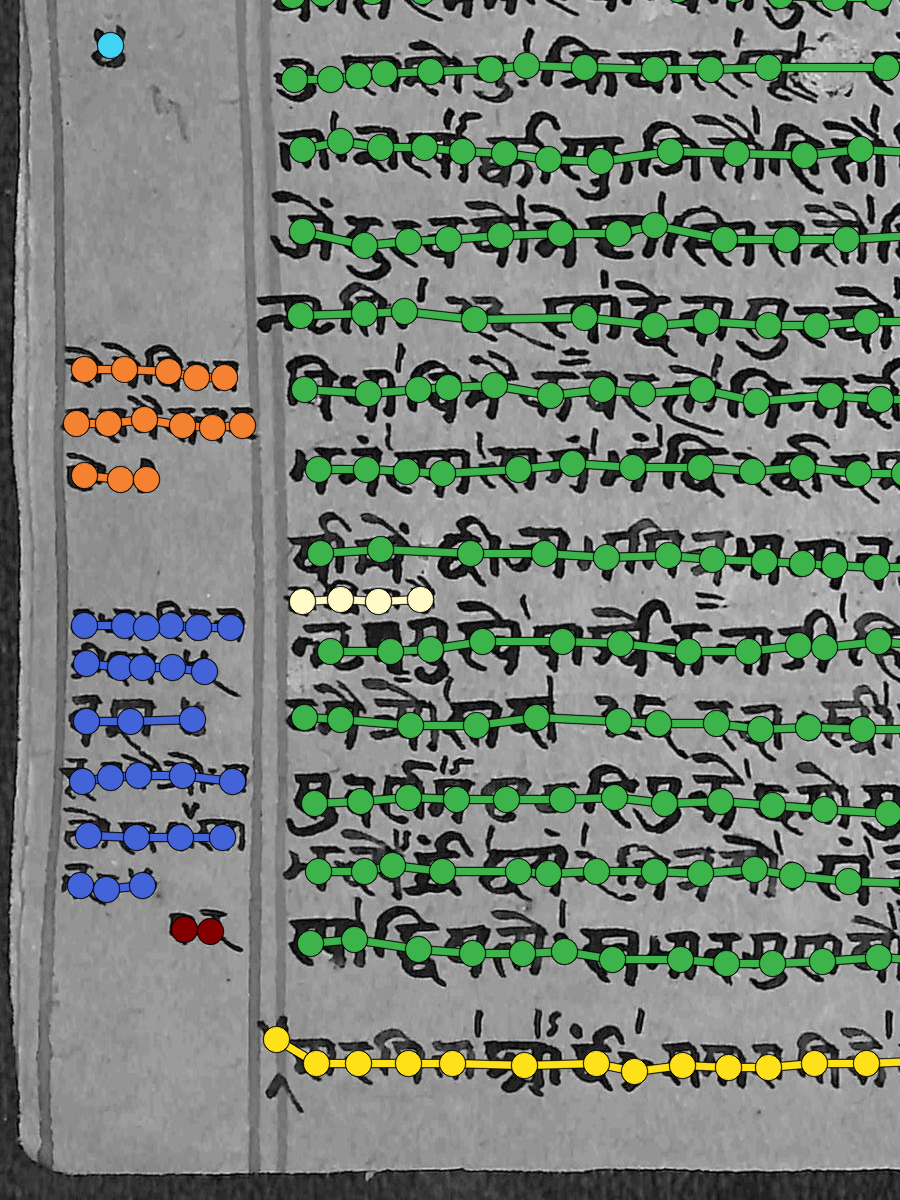
\includegraphics[width=\linewidth]{experiments/annotation_viz/output/page_10_text_regions.png}
    \caption{Regions annotation}
  \end{subfigure}\hfill
  \begin{subfigure}[t]{0.245\textwidth}
    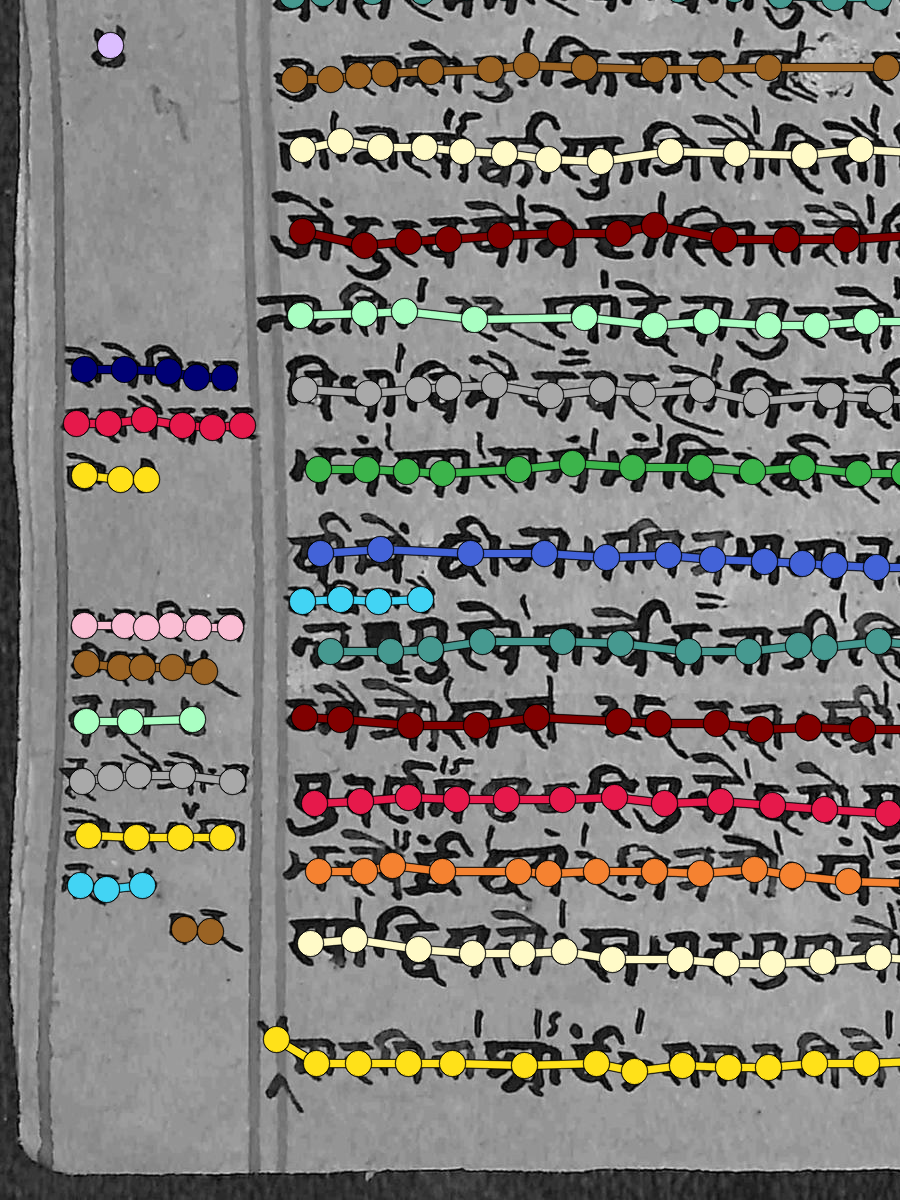
\includegraphics[width=\linewidth]{experiments/annotation_viz/output/page_10_text_lines.png}
    \caption{Text-line annotation}
  \end{subfigure}\hfill
  \begin{subfigure}[t]{0.245\textwidth}
    
\includegraphics[width=\linewidth]{experiments/annotation_viz/output/page_10_unicode_text.png}
    \caption{Unicode annotation}
  \end{subfigure}
  \caption{Bottom-left crop of page 10 showing the four annotation views.}
  \label{fig:page-10-annotation-views}
\end{figure*}
